\documentclass[12pt]{article}
\usepackage{hyperref}
\usepackage[warn]{mathtext}
\usepackage[T2A]{fontenc}
\usepackage[utf8]{inputenc}
\usepackage[russian]{babel}
\usepackage{cite}
\usepackage{amsfonts}
\usepackage{lineno}
\usepackage{subfig}
\usepackage{graphicx}
\usepackage{xcolor}
\usepackage{bm}
\usepackage{graphicx}
\usepackage{amssymb}
\usepackage{hyperref}
\usepackage[left=2cm,right=2cm,top=2cm,bottom=2cm]{geometry}

\DeclareGraphicsExtensions{.png,.jpg}
\date{14 сентября 2021 г.}
\author{Карцев Вадим}
\title{Лабораторная работа 2.1

Опыт Франка-Герца}

\begin{document}

\maketitle

\section{Теоретическая справка}
  Опыт Франка-Герца доказывает существование дискретных уровней энергии атома.

  В опыте используется трехэлектродная лампа, наполненная разреженным
  одноатомным газом.

  \begin {figure}[h!]
    \begin{minipage}[h]{0.49\linewidth}
        \center{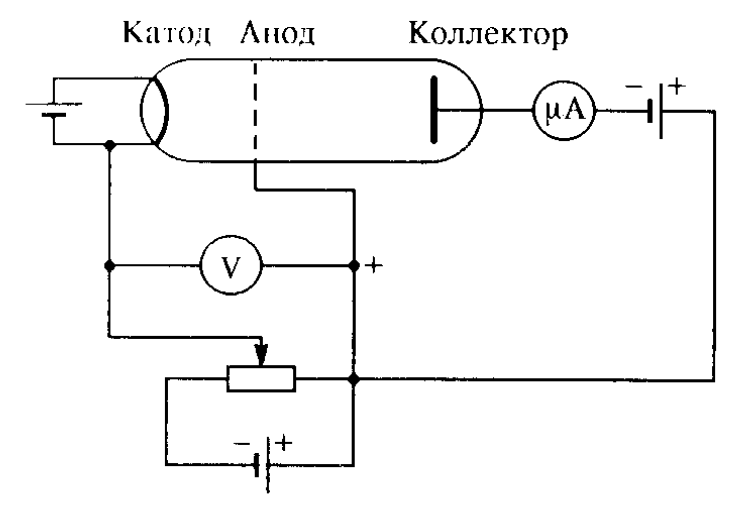
\includegraphics[width = 9cm]{ustanovka.png}}\\
        Рис 1. Схема установки
    \end{minipage}
    \begin{minipage}[h]{0.49\linewidth}
        \center{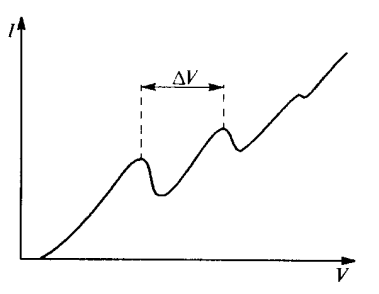
\includegraphics[width = 7cm]{scheme_plot.png}}\\
        Рис 2. Схематическая зависимость тока на коллекторе от разницы потенциалов между анодом и катодом
    \end{minipage}
    \label {fig:image1}
  \end {figure}

  Увеличивая разницу потенциалов между анодом и катодом мы увеличиваем энергия электронов.
  Пока энергии недостаточно для перевода атомов в возбужденное состояние, соударения будут практически
  упругими, т.к. масса электронов мала по сравнению с массой атомов. При дальнейшем увеличении энергии
  электронов начинает хватать для возбуждения или ионизации атомов газа и часть электронов теряет свою энергию
  при соударениях. Таким электронам не хватает энергии преодолеть задерживающее напряжение между анодом и
  коллектором и наблюдается резкое падение тока на последнем.


\end{document}
